\documentclass[reqno]{amsart}

\usepackage{amsfonts,latexsym,amsthm,amssymb,amsmath,amscd,euscript,bm}
\usepackage[sc]{mathpazo}
\usepackage[margin = 2cm]{geometry}
\usepackage{enumitem}
\usepackage{hyperref}
% sets numbering of enumerate to a, b, c, ...
\renewcommand{\theenumi}{\alph{enumi}}

% Theorems, propositions, etc.
\newtheorem{theorem}{Theorem}
\newtheorem{proposition}[theorem]{Proposition}
\newtheorem{lemma}[theorem]{Lemma}
\newtheorem{corollary}[theorem]{Corollary}

\theoremstyle{definition}
\newtheorem{definition}[theorem]{Definition}
\newtheorem*{claim}{Claim}

\theoremstyle{remark}
\newtheorem*{remark}{Remark}
\newtheorem*{notation}{Notation}
\newtheorem*{example}{Example}

\usepackage{tikz-cd}



% Math blackboard font
\newcommand{\nc}{\newcommand}
\nc{\on}[1]{\operatorname{#1}}

\nc{\R}{\mathbb R}
\nc{\C}{\mathbb C}
\nc{\Q}{\mathbb Q}
\nc{\Z}{\mathbb Z}
\nc{\N}{\mathbb N}
\nc{\HH}{\mathbb H}
\nc{\DD}{\mathbb D}
\nc{\TT}{\mathbb T}
\nc{\EE}{\mathbb E}
\nc{\PP}{\mathbb P}

\nc{\cT}{\mathcal T}
\nc{\cA}{\mathcal A}
\nc{\cM}{\mathcal M}
\nc{\cR}{\mathcal R}
\nc{\cB}{\mathcal B}
\nc{\cG}{\mathcal G}
\nc{\cD}{\mathcal D}
\nc{\cS}{\mathcal S}
\nc{\cF}{\mathcal F}
\nc{\cL}{\mathcal L}
\nc{\cE}{\mathcal E}

\nc{\diam}{\operatorname{diam}}
\nc{\del}{\partial}
\nc{\osc}{\operatorname{osc}}
\nc{\inter}{\mathrm{o}}
\nc{\close}[1]{\overline{#1}}
\nc{\supp}{\operatorname{supp}}
\nc{\BV}{\operatorname{BV}}
\nc{\Per}{\operatorname{Per}}
\nc{\loc}{\text{loc}}
\nc{\Lip}{\operatorname{Lip}}
\nc{\ACL}{\operatorname{ACL}}

% Why the f*** would you ever use \epsilon
\renewcommand{\epsilon}{\varepsilon}
\renewcommand{\emph}{\textsc}
\renewcommand{\Re}{\operatorname{Re}}
\renewcommand{\Im}{\operatorname{Im}}
%inverse Fourier transform widecheck
\DeclareFontFamily{U}{mathx}{\hyphenchar\font45}
\DeclareFontShape{U}{mathx}{m}{n}{
      <5> <6> <7> <8> <9> <10>
      <10.95> <12> <14.4> <17.28> <20.74> <24.88>
      mathx10
      }{}
\DeclareSymbolFont{mathx}{U}{mathx}{m}{n}
\DeclareFontSubstitution{U}{mathx}{m}{n}
\DeclareMathAccent{\widecheck}{0}{mathx}{"71}

\let\vec\mathbf

% Title: change problem set number as needed
\title
{
	\emph{Manifolds}
} 

\author{Jason Zhao}
\date{\today}

\begin{document}
\maketitle
\tableofcontents

\section{Introduction}



\subsection{Manifolds}

A \emph{topological manifold} of dimension $n$ is a pair $(M, \cA)$, where $M$ is a second countable Hausdorff topological space and $\cA$ is an \emph{atlas}, a collection of \emph{coordinate charts} $\phi_\alpha : U_\alpha \to \R^n$ such that $U_\alpha \subseteq M$ form an open covering and $\phi_\alpha$ are homeomorphisms $U_\alpha \cong \phi_\alpha (U_\alpha)$. A \emph{smooth manifold} is a topological manifold such that the \emph{transition maps}
	\[ \phi_\beta \circ \phi_\alpha^{-1} : \phi_\alpha (U_\alpha \cap U_\beta) \to \phi_\beta (U_\alpha \cap U_\beta) \]
are smooth. 

\begin{example}
\leavevmode
\begin{itemize}
	\item $\R^n$ is a manifold with atlas consisting of the identity chart. 
	
	\item If $M$ is a manifold with charts $\phi_\alpha : U_\alpha \to \R^n$, then an open subset $U \subseteq M$ is also a manifold with charts $\phi_\alpha |_{U_\alpha \cap U} : U_\alpha \cap U \to \R^n$. 
	
	\item The general linear group $\mathsf{GL} (\R^n)$ is an open subset of the space of $n \times n$ matrices $\R^{n \times n}$ and hence is a manifold of dimension $n^2$. 
	
	\item If $M$ and $N$ are manifolds with charts $\phi_\alpha : U_\alpha \to \R^m$ and $\psi_\beta : V_\beta \to \R^n$ respectively, then the product $M \times N$ is a smooth $(m + n)$-dimensional manifold with charts $\phi_\alpha \times \psi_\beta : U_\alpha \times V_\beta \to \R^m \times \R^n$. 
	
	\item The $n$-sphere $S^n := \{ x \in \R^{n + 1} : |x| = 1 \}$ is a manifold with charts given by stereographic projection. 

\end{itemize}
\end{example}

Given a topological space $M$, two atlases $\cA = \{ \phi_\alpha : U_\alpha \to \R^n \}$ and $\cB = \{ \psi_\beta : V_\beta \to \R^n\}$ are \emph{compatible} if 
	\[  \psi_\beta \circ \phi_\alpha^{-1} : \phi(U_\alpha \cap V_\beta) \to \psi_\beta (U_\alpha \cap V_\beta) \]
is smooth for all $\alpha$ and $\beta$, i.e. $\cA \cup \cB$ defines an atlas. Compatibility defines an equivalence class on atlases, and we refer each class as a \emph{smooth structure}. The canonical representative of the smooth structure is the \emph{maximal atlas} $\cA_{\text{max}}$, the atlas such that if $\cA \sim \cA_{\text{max}}$, then $\cA \subseteq \cA_{\text{max}}$. 

\begin{remark}
	$S^1$ has only one smooth structure, while $S^7$ has several smooth structures. The \textit{smooth Poincare conjecture} on enumerating the smooth structures of $S^4$ remains open. 
\end{remark}

A map $f: M \to N$ between manifolds is \emph{smooth} if for any $p \in M$ there exist coordinate charts $\phi_\alpha: U_\alpha \to \R^m$ and $\psi_\beta : V_\beta \to \R^n$ such that $p \in U_\alpha$ and $f(p) \in V_\beta$ and 
	\[ \psi \circ f \circ \phi_\alpha^{-1} : \phi_\alpha (U_\alpha) \to \psi_\beta (V_\beta) \]
is smooth. We say $f$ is a \emph{diffeomorphism} if there exists a smooth inverse $f^{-1} : N \to M$. 

\subsection{Submersions, immersions and embeddings}



\begin{theorem}[Inverse function theorem]
	Let $U, V \subseteq \R^n$ be open, and suppose $f: U \to V$ is a $C^1$-function. If $df(x) : \R^n \to \R^n$ is a linear isomorphism, then there exist neighborhoods $U_x \subseteq U$ of $x$ and $V_{f(x)} \subseteq V$ of $f(x)$ such that $f_{|U_x}: U_x \to V_{f(x)}$ is a diffeomorphism. 
\end{theorem}

\begin{theorem}[Submersion theorem]
	Let $M$ and $N$ be manifolds of dimension $m$ and $n$ respectively such that $m \geq n$, and suppose $f: M \to N$ is a submersion. Then for each $p \in M$ there exist local coordinates $x$ and $y$ such that 
		\[ (x_1, \dots, x_m) \mapsto (x_1, \dots, x_n). \]
\end{theorem}

\begin{proof}
	
\end{proof}

\begin{corollary}
	Let $f: M \to N$ be a submersion, and suppose $y \in N$, then $f^{-1} (y)$ can be given the structure of a manifold. 
\end{corollary}

\begin{proof}
	
\end{proof}

\begin{example}
	The circle $S^1 \subseteq \R^2$ can be given the structure of a manifold via the submersion 
		\[ f(x, y) := x^2 + y^2 \]
\end{example}

\section{Tangent space}

Given a manifold embedded in Euclidean space, there is a clear extrinsic notion of a \emph{tangent space} of the manifold at a point $p$. We aim towards an intrinsic definition to generalise this notion of a tangent space $T_p M$ for an arbitrary manifold $M$ at a point $p \in M$. 

\begin{figure}[h]
	\begin{center}
		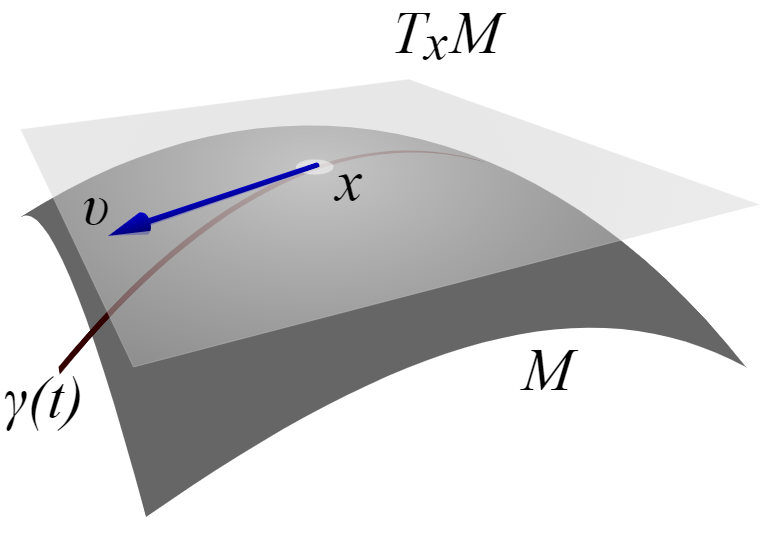
\includegraphics[scale =0.5]{tangent}
		\caption{Visual representation of the tangent space at a point $x \in M$ along with a tangent vector $v \in T_p M$, which in our first definition represents the ``velocity'' of a curve through $x$. }
	\end{center}	
\end{figure}

\subsection{Tangent curves}

The most intuitive and yet technically cumbersome definition of a tangent vector at $p \in M$ is as the \textit{velocity} of a curve passing through $p$. More precisely, let $\gamma, \eta : (-1, 1) \to M$ be smooth curves such that $\gamma(0) = \eta(0) = p$. We write the equivalence relation $\gamma \sim \eta$ if and only if 
	\[ f \circ \gamma = f \circ \eta + O(t^2) \]
for all $f \in C^\infty(U)$ where $U \subseteq M$ is a neighborhood of $p$. The tangent space $T_p^{(1)} M$ is the space of such curves up to the equivalence relation. We use local coordinates $x : U \to \R^n$ on a neighborhood of $p$ to endow $T^{(1)}_p M$ with a real vector space structure, defining
	\begin{align*}
		dx_p : T^{(1)}_p M 
			&\to \R^n, \\
		\gamma 
			&\mapsto \frac{d}{dt}(x \circ \gamma) (0).
	\end{align*}
This forms a well-defined bijection, so $T^{(1)}_p M$ inherits an $n$-dimensional real vector space structure from $\R^n$. 
	
\subsection{Derivations}

	Recall in Euclidean space we can identify a vector with its directional derivative, which is a linear map acting on smooth functions satisfying the product rule. To make precise this view, we need to briefly introduce some \textit{sheaf theory}. Let $U, V \subseteq M$ be neighborhoods of $p$ and suppose $f \in C^\infty (U)$ and $g \in C^\infty (V)$. We write the equivalence relation $f \sim g$ if and only if 
		\[ f_{|W} = g_{|W}  \]
	for some neighborhood $W \subseteq U \cap V$ containing $p$. The \textit{germ of smooth functions} $C^\infty (p)$ is the algebra of smooth functions up to the equivalence relation. Abstracting the directional derivative, a \emph{derivation} at $p$ is a linear map $X: C^\infty (p) \to \R$ satisfying the product rule
		\[ X(fg) = X(f) g(p) + f(p) X(g). \]
	The tangent space $T^{(2)}_p M$ is the space of derivations at $p$. There is a clear real vector space structure.
	
	\begin{lemma}
		The tangent space $T^{(2)}_p M$ has dimension $n$. 
	\end{lemma}
	
	\begin{proof}
	We use local coordinates $x^1, \dots, x^n$ to show that the dimension is $n$. Observe that $\tfrac{\partial}{\partial x^i}$ are linearly independent derivations satisfying $\tfrac{\partial}{\partial x^i} (x^j) = \delta_{ij}$, we want to show that they span $T^{(2)}_p M$. Let $X$ be a derivation, and it suffices to show
		\[ Y := X - \sum_{j = 1}^n X(x^j) \frac{\partial}{\partial x^j} \]
	is zero. By Taylor's theorem any $f \in C^\infty (p)$ can be written as $f = a + \sum_i a_i x^i + \sum_{ij} a_{ij} x^i x^j$. It follows that $Y(f) = 0$, as the quadratic and constant terms vanish by the product rule,  and the linear terms vanish by $Y(x^i) = 0$ from construction. 
	\end{proof}
	
	\begin{proposition}
		The map $\Phi: T^{(1)}_p M \to T^{(2)}_p M$ defined by 
			\[ \gamma \mapsto (X : f \mapsto (f \circ \gamma)' (0)) \]
		forms a well-defined linear isomorphism. 
	\end{proposition}

	\begin{proof}
	Linearity follows from the chain rule, 
		\begin{align*}
			(f \circ (\gamma + \eta))' (0) 
				&= (f \circ x^{-1} \circ x \circ (\gamma + \eta))' (0) = (f \circ x^{-1})' (x(p)) (x \circ (\gamma + \eta))' (0) \\
				&= (f \circ x^{-1})'(x(p)) \left[ (x \circ \gamma)' (0) + (x \circ \eta)' (0) \right] = (f \circ \gamma)'(0) + (f \circ \eta)' (0).
		\end{align*}	
	To show $\Phi$ is well-defined, recall that $\gamma_1 \sim \gamma_2$ if and only if $(f \circ \gamma_1) (t) =  (f \circ \gamma_2 )(t) + O(t^2)$ for every $f \in C^\infty (p)$. It follows that
		\[ (f \circ \gamma_1)' (0) - (f \circ \gamma_2)' (0) =  \lim_{t \to 0} \frac{(f \circ \gamma_1)(t) - (f \circ \gamma_2) (t)}{t} = \lim_{t \to 0} O(t) = 0.\]
	Conversely, we know from Taylor series that if $(f \circ \gamma_1)'(0) = (f \circ \gamma_2)'(0)$ then $(f \circ \gamma_1) (t) = (f \circ \gamma_2) (t) + O(t^2)$. This shows $\Phi$ is injective. Since $\dim T_p^{(1)} M = \dim T_p^{(2)} M = n$, we conclude $\Phi$ is a linear isomorphism. 
	\end{proof}
	
	
	\subsection{Cotangent space}
	
	Towards algebraic geometry, our third definition of the tangent space $T^{(3)}_p M$ will be as the dual of the \emph{cotangent space} $T^*_p M := \cF_p / \cF_p^2$, where $\cF_p \subseteq C^\infty (p)$ is the ideal of functions that vanish at $p$. By construction, the cotangent space is a quotient real vector space.

	
	\begin{proposition}
		Every derivation $X \in T^{(2)}_p M$ factors through $\cF_p^2$ to an induced map $\widetilde X \in T^{(3)}_p M$, and moreover the map $\Psi: T^{(2)}_p M \to T^{(3)}_p M$ defined by 
			\[ X \mapsto \widetilde X\]
		forms a well-defined linear isomorphism. 	
	\end{proposition}
	
	\begin{proof}
	We first show $X$ factors through $\cF_p^2$, i.e. $\cF_p^2 \subseteq \ker X$. Indeed, for any $f, g \in \cF_p$, the product rule gives
		\[ X(fg) = X(f) \cdot g(p) + f(p) \cdot X(g) = 0. \]
	To check $\Psi$ furnishes a linear isomorphism, we need to show bijectivity. It will be convenient to decompose $C^\infty (p)$ into $\cF_p$ the smooth functions that vanish at $p$ and $\mathcal C$ the constant functions. Indeed, $f - f(p) \in \cF_p$ for any $f \in C^\infty (p)$, and, if $f$ is both constant and vanishes at $p$, then $f \equiv 0$. Thus
		\[ C^\infty(p) = \cF_p \oplus \mathcal C. \]
	Recall that derivations vanish on constants $\mathcal C$. Moreover, if $\widetilde X \equiv 0$, then $X$ vanishes on $\cF_p$ and therefore $X \equiv 0$. This proves injectivity. For surjectivity, let $D: \cF_p /\cF_p^2 \to \R$ be a map in the cotangent space, define the linear map $X : C^\infty(p) \to \R$ by 
		\[ X(f + c) := D(f) \]
	for $f \in \cF_p$ and $c \in \mathcal C$. By construction, $X$ vanishes on $\cF_p^2$ and the constants, so for any $f, g \in C^\infty_p$, 
		\[ 0 = X((f - f(p))(g - g(p))) = X(fg) -  f(p) \cdot X(g) - g(p) \cdot X(f) \]	
	which shows that $X$ satisfies the product rule and therefore is a derivation. Moreover, by construction $\widetilde X = D$, which proves $\Psi$ is surjective. 
	\end{proof}

\section{Partition of unity}

\begin{claim}
		$M$ is locally compact, that is, every point has an open neighborhood with compact closure. Let $p \in M$ and $x$ be local coordinates around $p$. Since $\R^m$ is locally compact, let $G \subseteq \R^m$ be an open neighborhood about $x(p)$ which has compact closure. Since $x$ is a homeomorphism, $x^{-1} (G)$ is an open neighborhood of $p$ with compact closure. 
	\end{claim}
	
	\begin{claim}
		$M$ admits a countable covering by open sets with compact closure. Since $M$ is second countable, there exists a countable basis $\{ V_i \}_{i \in \N}$ for the topology. Let $K_p \subseteq M$ be an open neighborhood about $p \in M$ with compact closure, then 
			\[ K_p = \bigcup_{V_i \subseteq K_p} V_i. \]
		Since closed subsets of compact sets are compact, each $V_i$ has compact closure. Re-index such that $\{V_i\}_{i \in \N}$ is the sub-collection satisfying $V_i \subseteq K_p$ for some $p \in M$.
	\end{claim}
	
	\begin{claim}
		There exists a locally finite covering of $M$ by open sets with compact closure. Set $G_1 = V_1$ and let $j_k$ be the smallest positive integer satisfying
			\[ \close{G_{k - 1}} \subseteq \bigcup_{i = 1}^{j_k} V_i.  \]
		Define recursively for $k > 1$ 
			\[ G_k = \bigcup_{i = 1}^{j_k} V_i. \]
		Observe that $\{G_k\}_{k \in \N}$ is an ascending sequence of open sets with compact closure and form a covering of $M$. It follows that $\{ W_k \}_{k \in \N}$ defined by 
			\[ W_k = V_k \setminus \close{V_{k - 2}}\]
		is also a covering of $M$ by open sets with compact closure. Let $k \in \N$ be the smallest integer satisfying $p \in V_k$. By construction, $W_k$ only intersects $W_{k - 1}$ and $W_{k + 1}$, so the cover is locally finite. 
	\end{claim}
	For $p \in M$, we can find a largest integer $k_p \in \N$ and index $\alpha_p$ satisfying $p \in W_{k_p} \cap U_{\alpha_p}$. Choose a coordinate system $x: O_p \to \R^n$ about $p$ with $O_p$ chosen sufficiently small such that 
		\[ O_p \subseteq W_{k_p} \cap U_{\alpha_p}.\]
	Let $B_r \subseteq x(O_p)$ be an open ball of radius $r$ about $x(p)$. There exists a smooth bump function $\phi: \R^n \to \R$ supported on $B_r$. Define a non-negative smooth map $\psi_p$ on $M$ supported on $O_p$ by
		\[
			\psi_p = 
				\begin{cases}
					\phi \circ x, 	&\text{on $O_p$},\\
					0, 			&\text{elsewhere.}
				\end{cases}  
		\]
	Note $\close{V_k} \setminus V_{k -1}$ is compact, contained in $W_{k + 1} \cup W_k$ and forms a cover of $M$, so the open covering
		\[ \close{V_k} \setminus V_{k -1} \subseteq \bigcup_{p \in \close{V_k} \setminus V_{k - 1}} O_p \]
	admits a finite sub-cover, indexed by $p_1, \dots, p_{n_k} \in \close{V_k} \setminus V_{k -1}$. This gives us a countable collection $\psi_{p_j}$ supported on $U_{\alpha_p}$ indexed over $k \in \N$ and $1 \leq j \leq n_k$, which we re-index as $\psi_j$ and define
		\[ \phi_j = \frac{\psi_j}{\sum_{i \in \N} \psi_{i}} \]
	where the sum in the denominator converges and is smooth since by construction the supports of $\psi_j$ are locally finite, so at any point in $M$ the $\psi_j$ in a neighborhood for all but finitely many $j$. Indeed, we have $p \in W_k$ for some $k \in \N$ and since only finitely many supports are contained in $W_{k - 1} \cup W_k \cup W_{k + 1}$, only finitely many supports are contained in $W_k$. 
	
	By construction, $\phi_j$ is a countable collection, each with compact support in some $U_\alpha$, locally finite, and satisfy $\sum \phi_j = 1$ pointwise. 	


\section{Embedding}

\subsection{Sard}

Earlier we proved that given a smooth map between manifolds $f: M \to N$, the fibers of the regular values of $f$ form embedded submanifolds of $M$. However, it is not known a priori whether these regular values exist. It turns out that Sard's theorem says that such regular values indeed do exist, and in fact they are \emph{generic}, in the following senses:

\begin{definition}
	Let $N$ be a smooth manifold. We say that a set $S \subseteq N$ has \emph{measure zero} if there exists a countable atlas $\{ (U_i, \phi_i) \}_{i \in \N}$ such that $\phi_i (U_i \cap S)$ has Lebesgue measure zero for each $i \in \N$. 
	
	More precisely, $S$ has measure zero if for every $\epsilon > 0$ and $i \in \N$, there exists a countable collection of rectangles $R_{i, j} = [a_{i, j, 1}, b_{i, j, 1}] \times \dots \times [a_{i, j, n}, b_{i, j, n}]$ covering $\phi_i (U_i \cap S)$ with total volume less than $\epsilon$, i.e.
		\[ \phi_i (U_i \cap S) \subseteq \bigcup_{j \in \N} R_{i, j}, \qquad \sum_{j \in \N} \prod_{k = 1}^n (b_{i, j, k} - a_{i, j, k}) < \epsilon. \]
\end{definition}

\begin{definition}
	Given a topological space $X$, a set $A \subseteq X$ is \emph{nowhere dense} if its closure has empty interior. We say $A$ is \emph{meagre} if it is the countable union of nowhere dense sets. The complement of a meagre set is \emph{comeagre}.
\end{definition}

\begin{remark}
	Not all measure zero sets are meagre and not all meagre sets are measure zero. Consider an enumeration of the rationals $\{q_k\}_{k \in \N} \subseteq \R$ and open intervals around each rational of radius $1/n2^k$, namely
		\[ U_{k, n} = \left( q_k - \frac{1}{n 2^k},  q_k + \frac{1}{n 2^k} \right). \]
	It is an easy exercise to show that a set is meagre if and only if the complement of its closure is a countable intersection of open dense sets. Since $\Q$ is dense in $\R$, we know $\bigcup_k U_{k, n}$ is open and dense as well with measure less than $2/n$. Then 
		\[ \bigcap_{n \in \N} \bigcup_{k \in \N} U_{k, n} \]
	is comeagre and has measure zero. By the Baire category theorem, comeagre sets in $\R$ are not meagre. 
\end{remark}

\begin{theorem}[Sard's theorem]
	The set of critical values for a smooth function $f: M \to N$ is meagre and has measure zero. 
\end{theorem}

\begin{proof}
	We will prove the measure zero result; meagreness follows a similar proof (see Peter Petersen's notes).  The definition of measure zero is local and we can always find a countable atlas via second countability, so we can assume without loss of generality that $M \subseteq \R^m$ and $N \subseteq \R^n$ are open subsets. 
	
	We proceed via induction on $m$ the dimension of the domain. The theorem clearly holds for $m = 0$, so we will assume that it holds for $m - 1$ and prove it for $m$. Let $C$ be the set of critical points and define
		\[ C_k = \{ x \in C : \partial^\alpha f (x) = 0 \text{ for all } |\alpha| \leq k \}.\]
	Notice that $C_k$ is closed in $C$ by continuity of the partial derivatives. Moreover, $C$ is closed in $M$ since it is the zero set of the following continuous function 
		\[ x \mapsto \det (df(x) \cdot [df(x)]^t). \]
	\begin{claim}
		$f(C - C_1)$ has measure zero. If $x \in C \setminus C_1$, assume without loss of generality that the first partial of the first coordinate does not vanish, i.e. $\partial f_1 / \partial x_1 (x) \neq 0$. We define the smooth map $g: \R^m \to \R^m$ by 
			\[ g(x_1, \dots, x_m) = (f_1 (x_1, \dots, x_m) , x_2, \dots, x_m). \]
		By construction, $\det dg (x) = \partial f_1 / \partial x_1 (x)$, so $g$ locally a diffeomorphism at $x$. That is, there exist an open neighborhood $V \subseteq \R^m$ of $x$ and $V' \subseteq \R^m$ of $g(x)$ such that $g : V \to V'$ is a diffeomorphism. It follows from the chain rule that 
			\[  \]
		Moreover, $f \circ g^{-1} : V' \to N$ satisfies
			\[ (f \circ g^{-1})(x_1, \dots, x_m) = (x_1, f_2 \circ g^{-1} (x_1, \dots, x_m), \dots, (f_n \circ g^{-1})(x_1, \dots, x_m)). \]
			
			
	\end{claim}
	
	\begin{claim}
		$f(C_k - C_{k + 1})$ has measure zero. Our argument here is analogous to the previous case: if $x \in C_k \setminus C_{k + 1}$, there is a $k$-th order derivative of $f$, call it $\rho$, that vanishes however $\partial \rho /\partial x_1 (x) \neq 0$. Define $h(x) = (\rho(x), x_2, \dots, x_n)$.
		
		The argument is the same. 
	\end{claim}
	
	\begin{claim}
		$f(C_k)$ has measure zero for $k > m/n - 1$. By local coordinates we can characterise $f$ as a map on the $m$-cube $f: [-1,1]^m \to N$. 
		
		Let $S \subseteq M$ be a cube whose sides are of length $\delta$. If $k$ is sufficiently large, we prove that $f(C_k \cap S)$ has measure zero. Since $C_k$ can be covered by countably many such cubes, we are done. 
		
		From Taylor's theorem, the compactness of $S$, and the definition of $C_k$, we see that 
			\[ f(x + h) = f(x) + R(x, h) \]
		where $R(x, h)| < a|h|^{k + 1}$ for $x \in C_k \cap S$ and $x + h \in S$. Here $a$ is constant depending only on $f$ and $S$. 
	\end{claim}	
\end{proof}

\subsection{Whitney embedding theorem}

Thus far we have studied manifolds \textit{intrinsically}, using only information arising from the manifold itself. Introductory texts on differentiable manifolds often take the \textit{extrinsic} approach, taking manifolds as defined within Euclidean space and exploiting this external structure. Whitney's embedding theorem shows that in fact the extrinsic approach loses no generality in that every manifold embeds within a Euclidean space. 

\begin{theorem}[Weak Whitney embedding theorem]
	Let $M$ be a manifold of dimension $n$, then there exists an embedding $f: M \to \R^{2n + 1}$. 
\end{theorem}

\begin{remark}
	The strong Whitney embedding theorem states an embedding $f: M \to \R^{2n}$ exists. 
\end{remark}

In this section, $M$ is an $m$-dimension manifold. Our goal will be to prove Whitney's (weak) embedding theorem, that $M$ can be embedded into $\R^{2m + 1}$. 

\begin{enumerate}
	\item Show that every one-to-one immersion $M \to \R^n$ for $n > 2m + 1$ can be projected down to a one-to-one immersion $M \to \R^{n - 1}$, and so by induction $M \to \R^{2m + 1}$. 
	\item Prove Whitney embedding for compact manifolds. 
	\item Prove the existence of a one-to-one immersion $M \to \R^n$ for some $n > 2m + 1$ using the compact case and a partition of unity subordinate to a cover by precompact open sets. 
	\item Prove the existence of a proper function $M \to \R$. 
	\item Conclude the Whitney embedding theorem. 	
\end{enumerate}

\begin{lemma}
	Let $f: M \to \R^n$ be a one-to-one immersion for $n > 2m + 1$. Then there exists a one-to-one immersion $\tilde f : M \to \R^{2m + 1}$. 
\end{lemma}

\begin{proof}
	Let $\sigma: M \times M \times \R \to \R^n$ and $\tau: TM \to \R^n$ be the maps
		\[ \sigma(x, y, t) = t(f(x) - f(y)), \qquad \tau(x, v) = df (x)(v). \]
	By Sard's theorem, there exists a regular value $v \in \R^n$. The image of $\sigma$ has dimension at most $2m + 1$ and the image of $\tau$ has dimension at most $2m$, so $v$ is regular only if it is not in the image of $\sigma$ and $\tau$. Let $\pi : \R^n \to \R^{n - 1}$ be the orthogonal projection onto $v^\perp$. We claim that $\pi \circ f$ is a one-to-one immersion. 
	
	Suppose $(\pi \circ f) (x) = (\pi \circ f) (y)$, i.e. $\pi (f(x) - f(y)) = 0$. The kernel of $\pi$ is exactly the span of $v$, so there exists $t \in \R$ such that 
		\[ t(f(x) - f(y)) = v, \]
	contradicting the assumption that $v$ is not in the image of $\sigma$. Note that 
		\[ d(\pi \circ f) = \pi \circ df. \]
	So the kernel of $d(\pi \circ f)$ is exactly that of $df$. 
\end{proof}

\begin{theorem}[Whitney's (weak) embedding theorem]
	Given an $n$-dimensional manifold $M$, there exists and embedding $f: M \to \R^{2m + 1}$. 
\end{theorem}

\begin{proof}
	Assume $M$ is compact. We first prove that $M$ can be embedded into $\R^m$ for $m >> 1$. We first cover $M$ be finitely many rectangles $R_1, \dots, R_k$ neighborhoods of $p_1, \dots, p_k \in M$.  
		\[ R_i = [-1, 1]^n \]
	with $p_i$ taken to zero by the coordinate chart. Choose an even (symmetric) bump function $\phi: \R \to \R$ supported on $[-1, 1]$ and $\phi'(x) \neq 0$ on $(-1, 0) \cup (0, 1)$. Let 
		\[ \phi_\epsilon (x) = \phi(x - \epsilon), \qquad \phi_{- \epsilon} \phi(x + \epsilon). \]
	Suppose $n = 1$. Define 
		\[ g = (\phi_{-\epsilon}, \phi_\epsilon).\]
	Observe that $g(x) = 0$ if and only if $x\not\in (-1 - \epsilon, 1 + \epsilon)$ and $g$ is an immersion on $(-1 - \epsilon, 1 + \epsilon)$ and $g(x) = g(y)$ if and only if $x = y$. Thus $g$ is a one-to-one immersion. 
	Suppose $n = 2$. Let $\psi$ be a bump function supported on $(-1 - 2\epsilon, 1 + 2 \epsilon)$ and $\psi = 1$ on $(- 1 - \epsilon, 1 + \epsilon)$. Set
		\[ g(x_1, x_2) = (\phi_{-\epsilon}(x_1) \psi (x_2), \phi_\epsilon (x_1) \psi(x_2), \phi_{-\epsilon} (x_2) \psi(x_1), \phi_\epsilon (x_2) \psi(x_1)). \]
	It is not hard to show that $g$ is an embedding on $(-1 - \epsilon, 1 + \epsilon)^n$. General $n$ is clear. Let $\psi_1, \dots, \psi_{2nk}$ be the list of components of $g$ over all rectangles $R_1, \dots, R_k$. Then define $f: M \to \R^{2nk}$ by 
		\[ x \mapsto (\psi_1 (x), \dots, \psi_{2nk} (x)) \]
	This is well defined since each is compactly supported. The claim is that $f$ is an embedding. It is an immersion since locally it is an immersion. To show it is one to one, if they are in the same rectangles, we are done. If they are in different rectangles, then one is non-zero, the other is zero because support. 
\end{proof}

\begin{enumerate}	
	
	\item Set 
			\[ f = \sum_{i \in \N} i \phi_i. \]
		Since $\phi_i$ are smooth and the supports are locally finite, the function is smooth and non-negative. To show $f$ is proper it suffices to show that $f$ pulls back the intervals $[0, n]$ to pre-compact sets. Suppose $x \not\in V_i$ for all $i = 1, \dots, n$, then 
			\[ f(x) = \sum_{i > n} i \phi_i (x) > n \sum_{i > n} \phi_i = n \]
		where the last equality holds since the partition of unity has unit mass at each point. Thus $x \in V_k$ for some $k \leq n$ whenever $f(x) \leq n$, i.e. 
			\[ f^{-1}([0, n]) \subseteq \bigcup_{k =1}^n V_k. \]
		As each $V_k$ is precompact, their union and every subset of their union is precompact, as desired. 	
			
	\item By Whitney embedding, we can assume $M$ is embedded in some Euclidean space, say $\R^m$. Via translation, we can assume without loss of generality that $M$ does not contain the origin, so the map norm map $x \mapsto |x|$ is smooth on $M$. By theorem of G\&P, 
			\[ g_a (x) = |x| + a \cdot x \]
		is Morse for almost every $a \in \R^m$. Choose $a$ such that $g_a$ is Morse and $|a| < 1/2$. We claim that $g_a$ is proper. By Cauchy-Schwarz, $|a \cdot x| \leq |x|/2$, so the reverse triangle inequality gives
			\[ |g_a (x)| \geq \left| |x| - |a \cdot x| \right| \geq \frac{|x|}{2} \]
	
	\item We claim that there exists an injective immersion $M \to \R^{2n + 1}$. Set
			\[ M_i = f^{-1} ([i, i + 1]) \]
		each of which are compact and therefore be covered by finitely many coordinate charts $U_{i1}, \dots, U_{ik_i}$. Define a countable open covering of $M$ by 
			\[ N_i = (U_{i1} \cup \dots \cup U_{ik_i}) \cap f^{-1} ((i - 1/4, i + 1/4)). \]
		Observe that $\{N_i\}_{i \in \N}$ is locally finite; specifically, any $x \in M$ is contained in at most two $N_i$. Each $N_i$ is covered by finitely many coordinate charts, so by the compact case of Whitney's embedding theorem, there exists an injective immersion $\phi_i : N_i \to \R^{2n + 1}$. Let $\rho_i : M \to \R$ be a smooth bump function supported on $N_i$ and $\rho_i = 1$ on $M_i$. Define $\Phi: M \to \R^{4m + 3}$ by 
			\[ p \mapsto \left( \sum_{i \text{ odd}} \rho_i (p) \phi_i (p), \sum_{i \text{even}} \rho_i (p) \phi_i (p), f(p) \right). \]
		We claim that $\Phi$ is a well-defined injective immersion. Indeed, by our observation of local finiteness, in each sum all the terms vanish except for one pointwise. This shows smoothness of $\Phi$. Suppose $p_1, p_2 \in M$ satisfy $\Phi(p_1) = \Phi(p_2)$. Then there exists $i \in \N$ such that
			\[ f(p_1) = f(p_2) \in [i, i + 1]. \]
		Thus $p_1, p_2 \in M_i \subseteq N_i$ so by construction of $\Phi$ we have $\phi_i (p_1) = \phi_i (p_2)$. Each $\phi_i$ is injective, so $p_1 = p_2$. This proves injectivity. Fix $p \in M_i$ for some $i$ odd and $v \in T_p M$ non-zero, then 
			\[ d\Phi(p)(v) = (d\phi_i (p)(v), *, *), \]
		where $*$ denotes stuff we don't care about. As $\phi_i$ is an immersion, $d\phi_i (p)(v) \neq 0$, so $d\Phi(p)(v) \neq 0$. The proof for $i$ even is the same. An astute grader will remember that the trick to reduce the dimension of the codomain to $2n + 1$ holds for non-compact manifolds, so we obtain the desired injective immersion $\Phi: M \to \R^{2n + 1}$. We can assume $\Phi$ maps into the unit ball, i.e. $|g| < 1$, by composing with the diffeomorphism $\R^{2n + 1} \to B^{2n + 1}$
			\[ z \mapsto \frac{z}{1 + |z|^2}. \]
		From here we follow G\&P. Define $F: M \to \R^{2n + 1}$ by 
			\[ F(p) = (\Phi(x), f(x)). \]
		Since $\Phi$ is one-to-one and an immersion, so is $F$. For $a \in \R^{2n + 1}$, let $\pi: \R^{2n +1} \to \R^{2n + 1}$ be the orthogonal projection to $a^\perp$. By Sard we know that $\pi \circ F$ is an injective immersion for almost ever $a$, so fix 
			\[ a \neq (0, \dots, 0, \pm 1).\]
		We claim that $\pi \circ F$ is proper. It suffices to show for every $r > 0$ there exists $R > 0$ such that
			\[ \{ p \in M : |(\pi \circ F)(p)| \leq r \} \subseteq \{ p \in M : |f(x)| \leq R \}. \]
		Assume otherwise, then there exists $\{ x_k \}_{k \in \N} \subseteq M$ such that $|(\pi \circ F)(x_k)| \leq r$ but $f(x_k) \to \infty$. By definition of orthogonal projection, 
			\[ \frac{F(x_k) - (\pi \circ F)(x_k)}{f(x_k)} \in \on{span} a. \] 
		Since $\Phi$ is uniformly bounded on $M$ and $\pi \circ F$ is uniformly bounded on the sequence $\{x_k\}_{k \in \N}$, we have
			\[ \frac{F(x_k) - (\pi \circ F)(x_k)}{f(x_k)} = \left( \frac{\Phi(x_i)}{f(x_i)}, 1 \right) - \frac{(\pi \circ F)(x_k)}{f(x_k)} \overset{k \to \infty}{\longrightarrow} (0, \dots, 0, 1). \]
		However, $\on{span} a$ is a closed subspace of $\R^n$ that does not contain the north or south pole, so this is a contradiction. Thus $\pi \circ F : M \to \R^{2n + 1}$ is an injective proper immersion, i.e. an embedding. 
	
\end{enumerate}


\end{document}